\documentclass[main.tex]{subfiles}
\begin{document}
\section{Offset Robotic Arm}\label{sec:robotarmoffset} 
This section provides the complete worked example of the methodology, illustrating the process from selection of a mechanical system all the way to dynamical reduction. 

This example is adapted from \ref{sec:robotarm}, modified such that the actuated joint is offset from the centre of the block. This results in a coupling of the dynamics of the arm and the block--a much more interesting problem. Additionally, the actuator controlling the length of the arm is removed. This gives the system two degrees of underactuation, which is favourable for the dynamical reduction technique being explored.

\textbf{Description} Consider a massive body which rotates around a fixed point in space. A leg extends from the body, which can rotate relative to the body and change its length.
\begin{figure}[h]
    \centering
    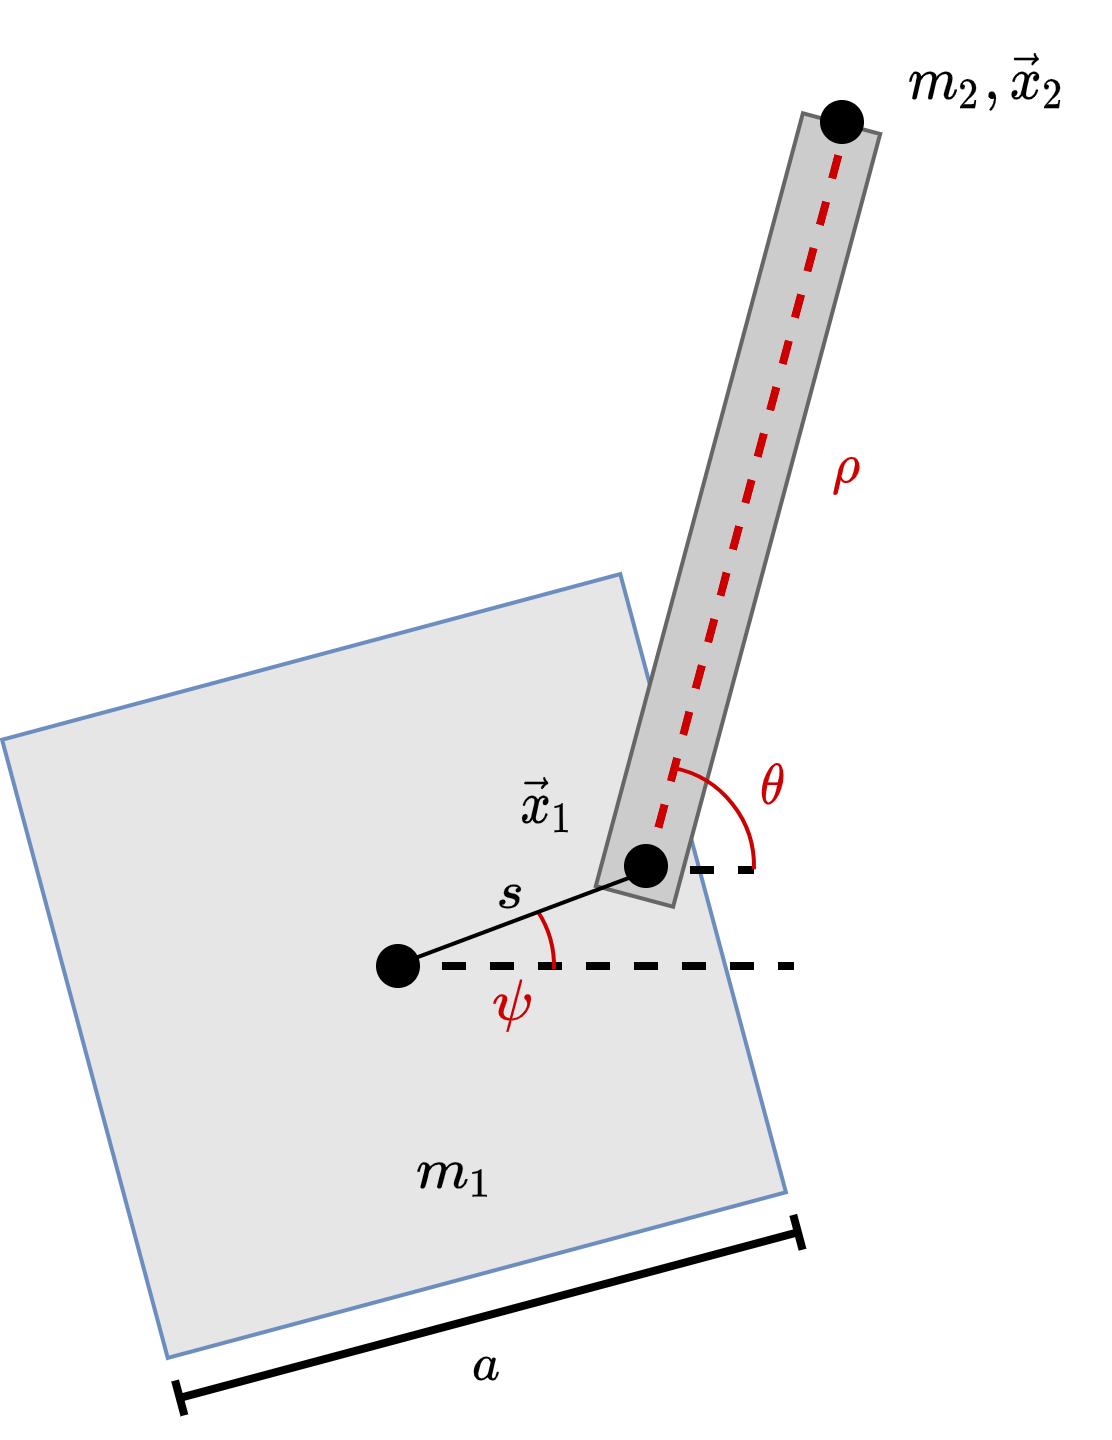
\includegraphics[width=0.5\textwidth]{assets/robot-arm.png}
    \caption{Offset robotic arm schematic diagram}
    \label{fig:rob-arm}
\end{figure}


\begin{enumerate}[(1)]
\item The smooth simple simple mechanical control system $(Q,\mathbb{G},F,P)$ is given by:
\begin{itemize}
    \item \textbf{Configuration space} $Q=\ree_{>0}\cross\mathbb{S}^1\cross\mathbb{S}^1$, with coordinates $q=(r,\theta,\psi)$
    \item \textbf{Kinetic metric} $\mathbb{G}=m(\dd r\otimes\dd r + r^2\dd\theta\otimes\dd\theta)+J\dd\psi\cross\dd\psi$
    \item \textbf{Actuation} $F=(\dd \theta,\dd \tau)$
    \item \textbf{Potential} In this example, there is no potential field: $\nabla P=(0,0,0)$. This is chosen to allow the existence of a symmetry in the system dynamics.
\end{itemize}
From the diagram of the system, it can be shown that the spatial coordinates are
\begin{align}
    \Vec{x}_1&=s\cos\psi\hat{x}+s\sin\psi\hat{y},\\
    \Vec{x}_2&=\Vec{x_1}+\rho\cos\theta\hat{x}+\rho\sin\theta\hat{y}.
\end{align}
The velocities are given by,
\begin{align}
    \dot{\Vec{x}}_1&=-s\dot\psi\sin\psi\hat{x}+s\dot\psi\cos\psi\hat{y},\\
    \dot{\Vec{x}}_2&=\dot{\Vec{x}}_1+(\dot\rho\cos\theta-\rho\sin\theta\cdot\dot\theta)\hat{x}+(\dot\rho\sin\theta+\rho\cos\theta\cdot\dot\theta)\hat{y}.
\end{align}
\item The system's Lagrangian depends on the kinetic energy of the solid body and of the point mass. There is no potential in this model.
\begin{align}
    \Lagr(q,\qd)=\frac{1}{2}\del{\frac{a^2}{12}m_1+s^2m_2}\dot{\psi}^2+\frac{1}{2}m_2\del{\dot\rho^2+\rho^2\dot\theta^2}+m_2s\del{\dot\rho\dot\psi\sin(\theta-\psi)+\psi\rho\dot\theta\cos(\theta-\psi)}.\label{eq:robarmofflagr}
\end{align}
\item From Equation \ref{eq:robarmofflagr}, the system's symmetry is found to be in the difference $\xi:=\theta-\psi$. 
 % We can therefore equivalently define the Lagrangian using $\xi$ (noting that the velocities $\dot q=(\dot\rho,\dot\theta,\dot\psi)$ are \textit{not} subject to this symmetry):
 % \begin{align}
 %     \Lagr(q,\dot q)&=\Lagr(\rho,\theta,\psi,\dot q)
 %     =\Lagr(\rho,\xi,\dot q).\label{eq:xilagrangian}
 % \end{align}
Define the left action of the Lie group $\mathbb{S}^1$ to be $\Phi:Q\cross \mathbb{S}^1\to Q$ to be the symmetry of the system, where the configuration space is $Q=\ree^+\cross \mathbb{S}^1\cross \mathbb{S}^1$.
%\todoformat[not sure which style to pick]
    \begin{align}
        %\Phi:\del{\pmqty{\rho\\\theta\\\psi},g}\mapsto\pmqty{\rho\\\theta+g\\\psi+g}.\\
        \Phi:\pmqty{\rho\\\theta\\\psi}\in Q,g\in G\mapsto\pmqty{\rho\\\theta+g\\\psi+g}\in Q.
    \end{align}
We can see that for all $g\in G$, this symmetry has no effect on $\xi$:
\begin{align}
    &\xi(q):=\theta-\psi,\\
    &\xi\del{\Phi(q,g)}=(\theta+g)-(\psi+g)=\theta+\psi+g-g=\xi(q).\ \checkmark
\end{align}
Since the Lagrangian's $\theta,\psi$ dependency can be expressed as a function of $\xi$, the Lagrangian is also invariant under the action of $\Phi$. This means one of $\theta,\psi$ can be considered \textit{cyclic}, which in turn means that there is an associated conserved quantity\cite[260]{marsden2013introduction}.
% . Bringing back our $\xi$-dependent Lagrangian from Equation \ref{eq:xilagrangian},
%     \begin{align}
%         \Lagr\del{\Phi(q,g),\dot q}
%     \end{align}
% SELECT VHCS ----------------------
\item {The} next step is to choose well-defined Virtual Holonomic Constraints that respect the symmetry defined above. 

The set of chosen VHCs $h(q)$ (Definition \ref{thm:regularvhc}) constrain the system to a submanifold $\mathcal{C}\subset Q$, with
    \begin{align}
        T_q\mathcal{C}&:=\Ker{\dhq}.\label{eq:tangentspaceqc}
    \end{align}
    This tangent space can equivalently be defined using the Ehresmann connection. Take $V(q)$ as the Vertical Vector Field defined by the direction of the symmetry:
    \begin{align}
        V(q):=&\pdv{\Phi}{g}=\pdv{}{g}\pmqty{\rho\\\theta+g\\\psi+g}=\pmqty{0\\1\\1}.\label{eq:dPhidg}
    \end{align}
    Together with an appropriate Horizontal Vector Field $H(q)$ of our choosing, we can get,
    \begin{align}
        T_q\mathcal{C}=\Span\cbr{V(q),H(q)}.
    \end{align}
    Now, we must select VHCs (and thereby also a constraint manifold $\mathcal{C}$) such that Equation \ref{eq:tangentspaceqc} holds true.

    The robot arm system has 3 degrees of freedom and 1 actuator, equating to $3-1=2$ degrees of underactuation. Since we plan to use this actuator to enforce the VHC, the constraint manifold should have $\dim\mathcal{C}=2$ remaining degrees of freedom.

    Select the following VHCs:
    \begin{align}
        h(q)&:=\theta-\psi\equiv 0,\\
        \dhq&=\pmqty{\pdv{h}{\rho}&\pdv{h}{\theta}&\pdv{h}{\psi}}=\pmqty{0&1&-1},\\
        \Ker{\dhq}&=\cbr{\pmqty{1\\0\\0},\pmqty{0\\1\\1}}.
    \end{align}
    Since $V(q)$ is seen in this basis (Equation \ref{eq:dPhidg}), it is natural to choose
    \begin{align}
    H(q)=\pmqty{1\\0\\0},
    \end{align}
    and their direct sum defines the fiber bundle $T\mathcal{C}=TV\oplus TH$.
    \item 
    The constrained dynamics are computed in two different methods. The first method involves a parametrization of the coordinates subject to the VHCs, and the second method uses Christoffel symbols.
    
    The Christoffel Symbols (Definition \ref{eq:christoffel}) of the constraint manifold $\Gammac{k}{ij}$ are computed in Matlab:
    \begin{align}
    \begin{split}
        \Gammac{1}{11}&=0\\
        \Gammac{1}{12}&=\rho\\
        \Gammac{1}{21}&=\rho\\
        \Gammac{1}{22}&=-L-\rho
    \end{split}
    \begin{split}
        \Gammac{2}{11}&=0\\
        \Gammac{2}{12}&=0\\
        \Gammac{2}{21}&=0\\
        \Gammac{2}{22}&=0
    \end{split}
    \end{align}
     
\end{enumerate}
\end{document}